% $Id: $
\documentclass[a4paper,11pt]{article}
\usepackage{a4wide}

\usepackage{amsmath,amsthm}
\usepackage{amsfonts}
% The following makes latex use nicer postscript fonts.
\usepackage{times}
\usepackage{subcaption}
\usepackage[english]{babel}
%\usepackage[colorlinks,urlcolor=blue,linkcolor=blue]{hyperref}
\pagestyle{headings}
\usepackage{vubtitlepage}
\usepackage{lmodern}

\usepackage[geometry]{ifsym}
%\usepackage[font=small,format=plain,labelfont=bf,up,textfont=it,up]{caption}
\renewcommand{\thefigure}{\thesection.\arabic{figure}}

\author{Filip Moons}
\title{Game Theory: Distributed Selfish Load Balancing on Networks}
\newtheorem{theorem}{Theorem}[section]
\newtheorem{lemma}[theorem]{Lemma}
\newtheorem{proposition}[theorem]{Proposition}
\newtheorem{conjecture}{Conjecture}
\newtheorem{example}[theorem]{Example}
\newtheorem{property}[theorem]{Property}
\newtheorem{definition}[theorem]{Definition}
\newtheorem{corollary}[theorem]{Corollary}
\newtheorem{remark}[theorem]{Remark}
\newtheorem{examples}[theorem]{Examples}
\newtheorem{remarks}[theorem]{Remarks}
\newtheorem{notation}[theorem]{Notation}
\setcounter{tocdepth}{5}
\newcommand{\N}{{\mathbb N}}
\newcommand{\Z}{{\mathbb Z}}
\newcommand{\Q}{{\mathbb Q}}
\newcommand{\R}{{\mathbb R}}
\newcommand{\C}{{\mathbb C}}
\newcommand{\HQ}{{\mathbb H}}
\renewcommand{\P}{{\mathbb P}}
\newcommand{\E}{{\mathbb E}}
\newcommand{\cost}{\text{cost}}
\newcommand{\Nash}{\text{Nash}}
\newcommand{\nash}{\text{nash}}
\newcommand{\opt}{\text{opt}}
\newcommand{\copt}{\cost(a_{\opt})}

%\newenvironment{proof}{\noindent{\bf Bewijs.}}{{\hfill $ \Box $}\vskip 4mm}

%\promotortitle{Promotor/Promotors}
\promotor{Prof. Dr. Ann Now\'{e}}
\advisors{}
\advisortitle{}
\addto\captionsenglish{\renewcommand*\abstractname{Abstract for non-mathematicians}}
\date{MEI 2006}
\faculty{Faculty of Science}
\advisortitle{}
\department{Department of Mathematics}
\reason{Bachelor Thesis I}

\date{January 2013}


\begin{document}
% Then english TitlePage
\maketitlepage
\newpage
\null\vspace{\fill}
\pagenumbering{roman}
\begin{abstract}
Explaining the subject of my Bachelor thesis to those who do not study either Mathematics or Computer Science isn't an easy task, but I can give an idea of the problem studied by giving an example. Imagine, for example, that there are only two roads from Paris to Brussels: road A \& road B. If you take road A you'll always drive 5 hours, independent from the usage of road A by other drivers (\emph{agents} is the more game theoretical word). If you take road B, the time you need depends of the number of other agents using road B: you'll drive $5\frac{x}{100}$ hours, with $x$ the number of agents, but also on this road the maximum time spend is 5 hours, so mathematically that becomes $\min(5, 5\frac{x}{100})$ hours. Because every agent acts selfish and rational, the result under this circumstances and with only this information will be that every agent will take at any time road B: with road A they drive always 5 hours, with road B there is a chance to get to Brussels in less time. But consider now the following situation: exact 100 agents decide at the same time to go to Brussels, that means that all of them will take road B and so everyone will drive 5 hours. It would be much better that 50 agents would take road A (and thus drive 5 hours) and the other 50 take road B (and drive $5\frac{50}{100} = 2.5$ hours), that would reduce the average time to $3.75$ hours! This kind of problems where the selfishness of agents reduce the power (load) of a general system take place in a wide range of real life problems: not only in traffic, but also in economics, politics and, that's more my interest, also in Computer Science: in a distributed system computers interact on a selfish base because there isn't a central computer that organizes the network. It's extremely interesting to study which solutions and/or which information these kind of agents (computers) need to know in order to reduce their selfishness and reach the optimal power of the distributed network.
\end{abstract}
\vspace{\fill}
\newpage

\tableofcontents
\newpage
\pagenumbering{arabic}

\section{Introduction}
Whenever a set of tasks should be executed on a set of resources, the problem of load balancing evidently arouses. We need to balance the load among the resources in order to exploit the available resources efficiently and fair.
\subsection{Why we need Game Theory}
 One of the most fundamental load balancing problems is \emph{makespan scheduling on uniformly related machines}. This problem is defined by $m$ machines with speeds $s_1,...s_m$ and $n$ tasks with weights $w_1,...,w_n$. Let $[n] = \{1,...,n\}$ be the set of tasks and $[m]$ the set of machines. Now, the problem is to find an assignment function $A: [n] \rightarrow [m]$ of the tasks to the machines that is as balanced as possible. The load of machine $j \in [m]$ under $A$ is defined as:
\begin{displaymath}
  \ell_j = \displaystyle\sum_{\substack{i \in [n] \\j = A(i)}}{\frac{w_i}{s_j}}
\end{displaymath}

The \emph{makespan} is defined as $$\max\limits_{j \in [m]}(\ell_j)$$

Now, of course, the objective is to minimize the makespan. When there is a central machine, it ins't that hard to design algorithms that compute a mapping A that minimizes the makespan. Suppose, however, that there is not a central machine that can enforce an efficient mapping of the tasks to the machines (e.g. in P2P Networks). This naturally leads to the following game theoretic setting in which we will be able to analyze what happens to the makespan if there is no global authority but selfish agents aiming at maximizing their individual benefit decide about the assignment of tasks. To understand the problem and it's solution, we first give the most important game theoretical results you'll need.

\section{Game Theory: Introducing Load Balancing Games}
Important note: This section doesn't aim to give the reader an introduction in Game Theory. Instead, it gives only the relevant results that the reader must know for understanding the rest of this paper.

\subsection{Strategic games}
\subsubsection{Definition}
\begin{definition}\cite{2}
A strategic game $\langle N, (A_i), \succeq_i\rangle$ consists of:
\begin{itemize}
  \item a finite set $N$  (the set of \textbf{players}),
  \item for each player $i \in N$ a nonempty set $A_i$ (the \textbf{set of actions} available to player i),
  \item for each player $i \in N$ a preference relation $\succeq_i$ on $A=\times_{j\in N}A_j$ (the \textbf{preference relation} of player i).
\end{itemize}
\end{definition}
\begin{remark}
Under a wide range of circumstances the preference relation  $\succeq_i$ of player $i$ in a strategic game can be represented by a \textbf{payoff function} $u_i: A \rightarrow \R$, in the sense that $u_i(a) \geq u_i(b)$ whenever $a \succeq_i b$. Sometimes this function is also called a utility function. A strategic game is then often denoted as $G = \langle N, (A_i), (u_i)\rangle$. In this paper, we assume that every strategic game has a payoff function, because the more general case is irrelevant for the subject studied.
\end{remark}


\subsubsection{Mixed and pure strategies}
A \emph{pure strategy} provides a complete definition of how a player will play a game. In particular, it determines the action a player will make for any situation he or she could face. Mathematically, an element $a = (a_1,...,a_n) \in A$ is called \emph{pure strategy profile}. The components $a_i$ of $a$ contain an action for each player at any stage of the game.

A \emph{mixed strategy} is an assignment of a probability to each action that is available to the player. This allows for a player to randomly select a pure strategy. Since probabilities are continuous, there are infinitely many mixed strategies available to a player, even if their strategy set is finite.

Of course, one can regard a pure strategy as a degenerated case of a mixed strategy, in which that particular pure strategy is selected with probability 1 and every other strategy with probability 0.

Let in a \emph{mixed strategy}, $\alpha_i(a_j)$ (with $a_j \in A_i$) denote the probability that player $i$ choose action $j$, thus: $\alpha_i(a_j) = \P[A_i = a_j]$. A \emph{mixed strategy profile} $$\alpha = \left(\alpha_i\right)_{i\in N}$$ specifies the probabilities for all players for all their possible actions. The probability of obtaining a specific pure strategy profile $a = (a_1,...,a_n)$ is:
$$\P[\alpha = a] = \displaystyle\prod_{i \in N} \alpha_i(a_i)$$
 We can now define the \emph{expected payoff} for player $i$ under a mixed strategy profile $\alpha$:
$$U_i(\alpha) = \displaystyle\sum_{a \in A}{\left(\prod_{j \in N}{\alpha_j(a_j)}\right) u_i(a)}$$
Or, by using the properties of the (discrete) expected value (we iterate over the pure strategy profiles $a \in A$)\footnote[1]{This notation is a little bit ambiguous, because in advanced game theory, also the payoff function may have a distribution. The reader must keep in mind that in this paper, payoff functions do not have a distribution.}:
$$U_i(\alpha) = \E[u_i(a)]$$
The set of all mixed strategy profiles in a strategic game for a specific player $i$ is denoted as $\Delta(A_i)$. Note that $(\alpha_i(a_1),...,\alpha_i(a_k),...)$ with the $a_j$'s the pure actions of player $i$ (thus $a_j \in A_i$) are the (vector)elements in $\Delta(A_i)$. The set of all mixed strategy profiles in a strategic game is denoted as $\Delta(A)$ and is defined as: $\Delta(A) = \Delta(A_1) \times ... \times \Delta(A_n)$ .


\subsubsection{Nash Equilibria}
One of the most fundamental concepts in game theory is that of Nash equilibrium. This notion captures a steady state of the play of a strategic game in which no player can improve his cost by unilaterally changing his strategy. Of course, we distinguish pure and mixed Nash Equilibria.

\begin{definition}(Pure Nash Equilibrium) \cite{6}
A pure strategy profile $a^* \in A$ is a \textbf{pure Nash Equilibrium} if for each player $i\in N$:
$$u_i(a_{-i}^*,a_i^*)) \geq u_i(a_{-i}^*, a_i) \;\;\;\; \forall a_i \in A_i$$
\end{definition}

\begin{definition}(Mixed Nash Equilibrium)\cite{10}
A mixed strategy profile $\alpha^*$ is a \textbf{mixed Nash Equilibrium} if for each player $i \in N$:
$$U_i(\alpha_{-i}^*,\alpha_i^*)) \geq U_i(\alpha_{-i}^*, \alpha_i) \;\;\;\; \forall \alpha_i$$
\end{definition}

\begin{remark}\label{herordening}
The notation $(a_{-i}^*, a_{i})$ for a pure strategy profile $a^*$ is a slight abuse of notation that is quite common in Game Theory, meaning that $a_i^* \in A_i$ and $a_{-i} \in A_1\times ... \times A_{i-1} \times A_{i+1} ... \times A_n$. The same holds for the mixed strategy profiles. It's important to realize that players have no exact order in a strategy profile, so they can always be re-ordered.
\end{remark}

Although there is not enough space to give a deep explanation of the concept of a Nash equilibrium, it's important to know that a Nash equilibrium is not necessary an optimal solution of a game. It's only a profile in which no player will benefit from changing his strategy on it's own.

\subsubsection{Theorem of Nash}
Now we have defined the concept of Nash Equilibrium, we can look at one of the most fundamental theorems in Game Theory: \emph{the Theorem of Nash}. This theorem states that every finite strategic game has at least one mixed Nash Equilibrium.

Nash proved his theorem in 1950 by using the Brouwer fixed point theorem. Later on, a lot easier version of the proof is found by using the Kakutani's fixed point theorem. However, the (one dimensional version of) the Brouwer fixed point theorem is much more familiar because it's proved in almost every intermediate Analysis course. Therefore, we will give the original proof of Nash.

\begin{definition}(Fixed point)\cite{111}
Let $X$ be a set and $f: X \rightarrow X$ a function. A point $x \in X$ is called a \textbf{fixed point} of $f$ if $f(x)=x$.
\end{definition}

\begin{property}(One dimensional version Brouwer fixed point theorem) \cite{111}
 Every continuous function $$f: [a,b] \rightarrow [a,b]$$  has a fixed point.
\end{property}
\begin{proof}
As the codomain of $f$ is $[a,b]$ it follows that the image of $f$ is a subset of $[a,b]$. Thus $f(a) \geq a$ and $f(b) \leq b$. Consider the function $$g: [a,b] \rightarrow \R: x \mapsto f(x) - x.$$
Then is $g$ also continuous and $g(a) \geq 0$ and $g(b) \leq 0$. By the theorem of Bolzano (see \cite{111}): $\exists c \in [a, b]: g(c) = 0$, but this means that $f(c) = c$.
\end{proof}
 The previous result is a very easy case of the Brouwer fixed point theorem. Proving the general theorem (see below) is very hard and falls behind the scope of this paper.
\begin{lemma}(Brouwer fixed point theorem)
Let $X$ be a non-empty, compact and convex set. If $f : X \rightarrow X$ is continuous, then there must exist $x \in X$ such that $f(x) = x$.
\end{lemma}

\begin{theorem}(Theorem of Nash)
Every finite strategic game has a mixed Nash equilibrium.
\end{theorem}

\begin{proof}
For every player $i$, let the set of actions $A_i$ be $\{a_{1}, ..., a_{m}\}$. For $1\leq i\leq n$. Let $\alpha$ be a mixed strategy profile of the the game and define $g_{ij}(\alpha)$ to be the gain for player $i$ form switching to his (pure) action $a_{j}$,:

$$g_{ij}(\alpha) = \max\{U_i(\alpha_{-i}, a_{j}) - U_i(\alpha),0\}$$

We can now define a map between mixed strategies of player $i$, $y:\Delta(A_i)\rightarrow \Delta(A_i)$ by

$$y_{ij}(\alpha) = \frac{\alpha_{i}(a_j)+g_{ij}(\alpha)}{1+\sum_{j=1}^{m}{g_{ij}(\alpha)}}$$

We now make three observations about this mapping:

\begin{itemize}
  \item For every player $i$ and his action $a_{j}$, the mapping $g_{ij}(\alpha)$ is continuous. This is due to the fact that $U_i(\alpha)$ is obviously continuous (it consists of the sum of products between a probability function and the continuous $u_i$), making $g_{ij}(\alpha)$ and consequently $y_{ij}(\alpha)$ continuous.

  \item For every player $i$, the vector $(y_{ij}(\alpha))_{j=1}^{m}$ is a distribution. This is due to the fact that the denominator of $y_{ij}(\alpha)$ is a normalization constant for any given $i$.


  \item Remember that $\Delta(A_i)$ has (vector)elements of the form $(\alpha_i(a_1),...,\alpha_i(a_k),...)$. Because the given strategic game is finite, we can identify $\Delta(A_i)$ with the set of vectors $(\alpha_i(a_1),...,\alpha_i(a_m))$, for which $\alpha_i(a_j) \geq 0 \;\; \forall j$ and $\sum^k_{j=1}{\alpha_i(a_j)} = 1$. We now proof that the set $\Delta(A_i)$ satisfies the conditions for the Brouwer fixed point theorem:
      \begin{itemize}
        \item The set $\Delta(A_i)$ is \emph{non-empty} by definition of a strategic game.
        \item To proof that the set $\Delta(A_i)$ is \emph{convex}, take $\vec{x} = (\alpha^x_i(a_1),...,\alpha^x_i(a_m))$ and $\vec{y} = (\alpha^y_i(a_1),...,\alpha^y_i(a_m))$ then $\vec{z} = \theta\vec{x} + (1 - \theta)\vec{y}$ for some $\theta \in [0,1]$ is in $\Delta(A_i)$ because $\vec{z}$ is also a mixed strategy for player $i$ (the sum of the components of $\vec{z}$ is 1).
        \item  The \emph{compactness} in $\R^k$ can be shown by proving that the set is closed and bounded. The set is bounded because $0 \leq \alpha_i(a_j) \leq 1$. To proof closeness in $\R^m$, we'll proof that the limit of every convergent sequence in $\Delta(A_i)$ is an element of $\Delta(A_i)$. Consider a convergent sequence in $\Delta(A_i): ((\alpha^n_i(a_1),...,\alpha^n_i(a_m))_n\rightarrow(\alpha^*_i(a_1),...,\alpha^*_i(a_m))$. Remember that a convergent sequence of vectors converges componentwise and that the addition is a continuous function, so:
            \begin{eqnarray*}
              \sum_{j=1}^m{\alpha^*_i(a_j)}  &=& \displaystyle\sum_{j=1}^m{\lim_{n\rightarrow\infty}{\alpha^n_i(a_j)}}\\
              &=& \displaystyle\lim_{n\rightarrow\infty}{\sum_{j=1}^k\alpha^n_i(a_j)}\\
              &=& \displaystyle\lim_{n\rightarrow\infty}{1}\\
              &=& 1
            \end{eqnarray*}
            this means that $(\alpha^*_i(a_1),...,\alpha^*_i(a_m))$ is also a mixed strategy for player $i$, but by definition of $\Delta(A_i)$, this limit belongs to $\Delta(A_i)$.
      \end{itemize}

\end{itemize}

Therefore $y$ fulfills the conditions of Brouwer's Fixed Point Theorem. Using the theorem, we conclude that there is a fixed point $\alpha^*$ for $y$. This point satisfies

$$\alpha^*_{i}(a_j) = \frac{\alpha^*_{i}(a_j)+g_{ij}(\alpha^*)}{1+\sum_{j=1}^{m}{g_{ij}(\alpha^*)}}$$

Notice that this is possible only in one of two cases. Either $g_{ij}(\alpha^*)=0$ for every $i$ and $j$, in which case we have an equilibrium (since no one can profit from switching their strategy). If this is not the case, then there is a player $i$ such that $g_{ij}(\alpha^*)>0$. This would imply,

$$\alpha^*_{i}(a_j)\left(1+\sum_{j=1}^{m}{g_{ij}(\alpha^*)}\right) = \alpha^*_{i}(a_j)+g_{ij}(\alpha^*)$$

or

$$\alpha^*_{i}(a_j)\left(\sum_{j=1}^{m}{g_{ij}(\alpha^*)}\right) = g_{ij}(\alpha^*)$$.

This means that $g_{ij}(\alpha^*)=0$ if and only if $\alpha^*_{i}(a_j)=0$, and therefore, $\alpha^*_{i}(a_j)>0 \implies g_{ij}(\alpha^*)>0$. However, this is impossible by the definition of $g_{ij}(\alpha^*)$. Recall that $U_i(\alpha)$ gives the expected payoff for a player under a mixed strategy $\alpha$. Therefore, it cannot be that player $i$ can profit from
`every' pure action in the support of $\alpha^*_i$ (with respect to $U_i(\alpha^*)$).

We are therefore left with the former possibility, i.e. $g_{ij}(\alpha^*)=0$ for all $i$ and $j$, implying a mixed Nash Equilibrium.
\end{proof}


\subsection{Congestion games}
\subsubsection{Definition}
Strategic games contains a wide range of games. We will now look at \emph{congestion games}: a specific kind of strategic games for which we can prove the existence of a pure Nash equilibrium. We will use this result for defining in the next section \emph{load balancing games}, a subclass of congestion games, this game is the one we'll need to handle the subject of this paper. Because we only need the theorem of the existence of a pure Nash equilibrium for congestion games, we will not take mixed strategies in consideration in this section.
\begin{definition}\cite{4,9}
A \textbf{congestion model} $(N, M, (A_i)_{i\in N}, (c_j)_{j\in M})$ is defined as follows:
\begin{itemize}
  \item a finite set $N$ of players. Each player $i$ has a weight (or demand) $w_i \in \N$,
  \item a finite set $M$ of facilities.
  \item For $i \in N$, $A_i$ denotes the set of strategies of player $i$, where each $a_i \in A_i$ is a non-empty subset of the facilities,
  \item For $j \in M, c_j$  is a cost function $\N \rightarrow \R$, $c_j(k)$ denotes the cost related to the use of facility $j$ under a certain load $k$;
\end{itemize}
\end{definition}
\begin{definition}\cite{2,4}
A \textbf{congestion game} associated with a congestion model is a strategic game with:
\begin{itemize}
  \item a finite set $N$ of players,
  \item for each player $i \in N$, there is a nonempty set of actions (strategies) $A_i$,
  \item the preference relation $\succeq_i$ for each player $i$ is defined by a payoff function $u_i: A \rightarrow \R$. For any $a \in A$ and for any $j \in M$, let $\ell_j(a)$ be \emph{the expected load on facility} $j$, assuming $a$ is the current pure strategy profile, so $\ell_j(a) = \sum_{\substack{i \in [n]\\j \in a_i}}{w_i}$ . Then the payoff function for player $i$ becomes: $u_i(a) = \sum_{j\in a_i} c_j(\ell_j(a))$.


\end{itemize}
\begin{remark}
Congestion models aren't always defined with the notion of weights of players (especially not in more economic game theory books). In those definitions, players have an equal weight. Those definitions match with ours if you give all players weight 1. Note that only the function $\ell_j(a)$ becomes much easier: it will just return the number of players using facility $j$ under a pure strategy profile $a$. From a computer scientific point of view, such definitions are not sufficient because players (\emph{tasks}) don't have the same weight. Watching the Eurovision Song Contest through a live stream is for example a much heavier task then sending an e-mail.
\end{remark}
\begin{remark}\label{defcj}
In order to preserve the generality in the definition of congestion games, note that we only stated that $c_j$ are cost functions, without the need to explicitly define them. This is sufficient in this stage of the paper, however, the subject studied will require explicit definitions for $c_j$. These are given in section \ref{expdefcj}.
\end{remark}
\end{definition}
\subsubsection{The existence of a pure Nash equilbrum}
Rosenthal proved in 1973 that every congestion game has a pure Nash Equilibrium. The proof of this statement uses the notion of a potential function. We will first define a potential function, give a concrete potential function for congestion games and proof that it holds the right properties. With this result we can finally proof the existence of a pure Nash Equilibrium in congestion games.

\begin{definition}
Consider a function $\Phi: A \rightarrow \R$  defined on the space of pure stategy profiles of a (strategic) game $G$. If player $i$ switches unilaterally from $a_i$ to $a_i^*$, taking us from profile $a$ to profile $a^*=(a_i^*, \vec{a_{-i}})$ and the following property holds:
$$\Phi(a) - \Phi(a^*) = u_i(a) - u_i(a^*) $$
then the function $\Phi$ is called a \textbf{potential function}.
\end{definition}



\begin{lemma}
The function
\begin{eqnarray*}
\Phi: A &\rightarrow& \R\\
a &\mapsto& \displaystyle\sum_{j=1}^{m}\displaystyle\sum_{k=1}^{\ell_j(a)} c_j(k)
\end{eqnarray*}
is a potential function for congestion games.
\end{lemma}

\begin{proof}(Rosenthal 1973)\cite{7,8}
In remark \ref{herordening} we already mentioned that players can be re-ordered. In particular, re-index player $i$ as player $n$ and vice versa.

Then, for $i' \in \{1,...,n\}$, define:
$$\ell_j^{i'}(a) = \displaystyle\sum_{\substack{l \in [1,...,i']\\j \in a_l}}{w_l} $$

Now, by using the commutativity, you can exchange the order of summation and become:
$$\Phi(a) = \displaystyle\sum_{i=1}^{n}\displaystyle\sum_{j\in a_i} c_j(\ell_j^i(a))$$

Denote that $\ell_j^n(a) = \ell_j(a)$, thus:
$$\displaystyle\sum_{j\in a_i} c_j(\ell_j^n(a)) = \displaystyle\sum_{j\in a_i} c_j(\ell_j(a)) = u_n(a)$$

So, if player $n$ switches from strategy $a_n$ to $a_n^*$, taking us from profile $a$ to profile $a^*=(a_n^*, \vec{a_{-n}})$ then:

\begin{align*}
\Phi(a) - \Phi(a^*) &= \!\left(\sum_{j\in a_1} c_j(\ell_j^1(a)) + ... + u_n(a) \!\right) - \!\left(\sum_{j\in a_1} c_j(\ell_j^1(a^*)) + ... + u_n(a^*) \!\right)\\
\intertext{By definition of $\ell_j^i$, this becomes (the $n$'th player doesn't count for $\ell_j^i$ with $i < n$):}
&= \left(\sum_{j\in a_1} c_j(\ell_j^1(a)) + ... + u_n(a) \right) - \left(\sum_{j\in a_1} c_j(\ell_j^1(a)) + ... + u_n(a^*) \right)\\
&= u_n(a) - u_n(a^*)
\end{align*}

We switched player $i$ with player $n$, so this holds for every player $i$.

\end{proof}

\begin{theorem}(Rosenthal 1973)\cite{7}\label{rosenthal}
Every congestion game has a pure Nash equilibrium.
\end{theorem}

\begin{proof}
Start from a random strategy vector $a$, and let repeatedly one player reduce it's costs. That means, that at each step $\Phi$ is reduced identically. Since $\Phi$ can accept a finite amount of values ($A$ is finite because it's the finite cartesian product of sets $A_i$ ($i \in \{1,...,n\}$), and every $A_i$ is finite because it's by definition a subset of the finite set of facilities $M$), this procedure will stop and reach a local minimum. At this point, no player can achieve any improvements, and we reach a pure \emph{Nash Equilibrium}.
\end{proof}



\subsection{Load balancing games}
\subsubsection{Definition}
Now we have introduced congestion games and proved that they always have a pure Nash Equilibrium, we take a closer look at a more specific kind of congestion games. Looking at the definition of a congestion game, it's immediately clear that this model is too general for giving a deeper understanding of the subject studied. Their is indeed a little problem with the actions (strategies) that a player can undertake: in a general congestion game, under a pure strategy profile $a$ the strategy of player $i$, $a_i$, consist of multiple facilities $j$. That means that the weight of a player (\emph{task}) counts for every function $c_j$ where $j \in a_i$. Of course, this is not realistic: a single task (\emph{player}) is not executed multiple times on different facilities. Therefore load balancing games are congestion games where the possible (pure) actions of players are singletons. So each $a_i = \{j\}$ ($i \in N, j \in M$) in a pure strategy profile $a \in A$. So, for every player $i$, $A_i \subset M$. In load balancing terminology, we use the terms \emph{machines} and \emph{tasks} instead of the terms facility and player.

\begin{definition}\cite{9}
A \textbf{load balancing game} is a congestion game based on a congestion model with:
\begin{itemize}
  \item a finite set $N$ of tasks (each task $i$ has a weight $w_i$,
  \item for each player $i \in N$, there is a nonempty set of machines $A_i$ with $A_i \subset M$. The elements of $A_i$ are the possible machines on which task $i$ can be executed.
  \item the preference relation $\succeq_i$ for each task $i$ is defined by a payoff function $u_i: A \rightarrow \R$. For any $a \in A$ and for any $j \in M$, let $\ell_j(a)$ be \emph{the expected load on machine} $j$, assuming $a$ is the current pure strategy profile ($\ell_j(a) = \sum_{\substack{i \in [n]\\j = a_i}}{w_i}$) . Then the payoff function for task $i$ becomes: $u_i(a) = c_{a_i}(\ell_{a_i}(a))$.
\end{itemize}
\end{definition}


\subsubsection{Payoffs and makespan for linear cost functions}\label{expdefcj}
Now we have defined \emph{load balancing games}, we can take a closer look at the subject studied. As already mentioned in remark \ref{defcj}, the cost functions in the previous section aren't explicitly defined. In this section we look at the situation where the cost functions $c_j$ for each machine $j$ are linear (thus of the form: $c_j(x) = \lambda_jx+\mu_j$ with $\lambda_j, \mu_j$ non-negative constants) and every machine has a certain \emph{speed} $s_j \in \N$.

\paragraph{Pure strategies}
In the most easy case, not only the players have a certain \emph{weight} $w_i \in \N$, also the machines have certain \emph{speed} $s_j \in \N$. Intuitively, such $s_j$ is the maximum amount of weight a machine can handle. The cost functions $c_j$ can then easily be defined as:
$$c_j(k) = \frac{k}{s_j}$$

 The \textbf{\emph{payoff functions}} become then:
$$u_i(a) = c_{a_i}(\ell_{a_i}(a)) =  \frac{\ell_{a_i}(a)}{s_{a_i}}$$
The \emph{\textbf{social costs}} of a pure strategy is denoted as $\cost(a)$ and is defined to be the \emph{\textbf{makespan}}, i.e. $$\cost(a)=\max_{j\in[m]}{c_j(\ell_j(a))} = \max_{j\in[m]}{\frac{\ell_{j}(a)}{s_{j}}}$$


\paragraph{Mixed strategies}
Of course, players may use mixed strategies. Now we can also define $\ell_j$ on mixed strategies: $\ell_j: \Delta(A) \rightarrow \R$, we will define $\ell_j(\alpha)$ as the \textbf{expected load}:

\begin{eqnarray*}
\ell_j(\alpha)  &=& \E[\ell_j(a)] \\
                &=&  \displaystyle\sum_{a \in A}{\left(\prod_{k \in N}{\alpha_k(a_k)}\right) \ell_j(a)}\\
                &=& \displaystyle\sum_{a \in A}{\left(\prod_{k \in N}{\alpha_k(a_k)}\right) \sum_{\substack{i \in [n]\\j = a_i}}{w_i} }\\
                &=& \displaystyle\sum_{a \in A}{\left(\prod_{k \in N}{\alpha_k(a_k)}\right) \sum_{i \in [n]}{w_i\delta_{a_i,j}}}\\
                 &=&  \displaystyle\sum_{a \in A}{\left(\P[\alpha = A]\right)\sum_{i \in [n]}{w_i\delta_{a_i,j}}}\\
                &=& \sum_{i \in [n]}{w_i}\P[A_i = j]\\
                &=& \sum_{i \in [n]}{w_i}\alpha_i(j)
\end{eqnarray*}

The \emph\textbf{{social cost of a mixed strategy profile}} is defined as the \emph\textbf{{expected makespan}}:
$$\cost(\alpha) = \E[\cost(a)] = \E\left[\max_{j\in[m]}\frac{\ell_j(a)}{s_{j}}\right]$$

For mixed strategies, the expected payoff for player $i$, denoted by $U_i$ is defined as:
\begin{eqnarray*}
U_i(\alpha) &=& \E[u_i(a)]\\
  &=&  \displaystyle\sum_{a \in A}{\left(\prod_{k \in N}{\alpha_k(a_k)}\right) \frac{\ell_{a_i}(a)}{s_{a_i}}}\\
  &=& \displaystyle\sum_{j \in [m]}{\frac{\ell_j(\alpha)}{s_j}\alpha_i(j)}
\end{eqnarray*}

From point of view of client $i$, the \emph{\textbf{expected cost on machine $j$}} under a mixed strategy profile $\alpha$, denoted by $U^j_i$, is:
\begin{eqnarray*}
U^j_i(\alpha) &=& \E[U_i(\alpha)|A_i=j]\\
  &=& \frac{w_i + \sum_{k\neq i}{w_k\alpha_k(j)}}{s_j} \\
  &=&  \frac{\ell_j(\alpha) + (1 - \alpha_i(j))w_i}{s_j}\\
\end{eqnarray*}
\subsubsection{An example with linear costs}
After more than 10 pages of theory, we give an easy example in which all the introduced concepts are contained.

Suppose that there are two identical machines that have both speed $1$ and four tasks, two \emph{small tasks} of weight $1$ and two \emph{large tasks} of weight 2. An optimal assignment would map a small and a large task to each of the machines so that the load on both machines is $3$. This assignment is illustrated in figure \ref{fig:a}.

Now consider a pure strategy profile $a$ that maps the two large tasks to the first machines and the two small tasks to the second machine as illustrated in figure \ref{fig:b}. This way, the first machine has a load of $4$ and the second machine has a load of $2$. Obviously, a small task cannot improve its cost by moving from the second to the first machine. A large task cannot improve its cost by moving from the first tot the second machine either as its cost would remain 4 if it does. Thus this pure strategy profile $a$ constitutes a \emph{pure Nash equilibrium} with $\cost(a)=4$. This is a beautiful example to show the already stated statement that Nash equilibria aren't mostly the optimal situations. Observe that all assigments that yield a larger makespan than 4 cannot be a Nash equilibrium as, in this case, one of the machines has a load of at least $5$ and the other has a load of at most $1$ so that moving any task from the former to the latter would decrease the cost of this task. Thus, for this instance of the load balancing game, the social cost of the worst pure Nash Equilibrium is 4.

Clearly, the worst mixed equilibrium cannot be better than the worst pure equilibrium as the set of mixed equilibria is a superset of the set of pure equilibria, but can it really be worse? Suppose that each task is assigned to each of the machines with probability $\frac{1}{2}$. This corresponds to a mixed strategy profile $\alpha$ with the $\alpha_i$'s being constant functions, $$\alpha = \bigg(\underbrace{\frac{1}{2}}_{\alpha_1}, \underbrace{\frac{1}{2}}_{\alpha_2}, \underbrace{\frac{1}{2}}_{\alpha_3}, \underbrace{\frac{1}{2}}_{\alpha_4}\bigg) $$
. The expected load on machine $j$ is thus:
$$\ell_j(\alpha) = \displaystyle\sum_{1\leq i \leq 4}{w_i\alpha_i(j)} = \frac{1}{2} + \frac{1}{2} + 1 + 1 = 3$$
It's important to notice that te expected cost of a task on a machine is larger than the expected load of the machine, unless the task is assigned with probability 1 to this machine. For example, if we assume that task 1 is a small task, then:
$$U_1^j = \frac{\ell_j(\alpha) + (1 - \alpha_1(j))w_1}{1} = 3 + \frac{1}{2} = 3.5$$
and, if task $3$ is a large task, then:
$$U_3^j = \frac{\ell_j(\alpha) + (1 - \alpha_3(j))w_3}{1} = 3 + \frac{1}{2}.2 = 4$$
For symmetry reasons, the expected cost of each task under the considered mixed strategy profile $\alpha$ is the same on both machines so that $\alpha$ is a \emph{mixed Nash equilibrium}. The social cost of this equilibrium, $\cost(\alpha)$, is defined to be the expected makespan, $\E[\cost(a)]$, of the random pure assignment $A$ induced by $\alpha$. The makespan, $\cost(a)$, is in fact a random variable. This variable can possibly take one of the four values $3, 4, 5$ or $6$. There are $2^4 = 16$ different assignments of four tasks to two machines. The number of assignments that yield a makespan of $3$ is $4$, 4 is 6, 5 is 4 and 6 (the loads of all possible assignments) is 2. Consequently, the social cost of the mixed Nash equilibrium is:
$$cost(\alpha) = \E[\cost(a)] = \frac{3.4 + 4.6 + 5.4+ 6.2}{16} = 4.25.$$
Thus mixed equilibria can, in fact, be worse than the worst pure equilibrium.
\begin{figure}
        \centering
        \begin{subfigure}{0.3\textwidth}
                \centering
                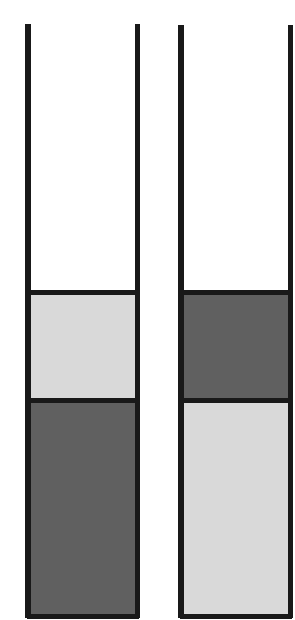
\includegraphics[scale=0.4]{figuura.pdf}
              \caption{Illustration of the optimal assignment}
                \label{fig:a}
        \end{subfigure}%
        ~ %add desired spacing between images, e. g. ~, \quad, \qquad etc.
          %(or a blank line to force the subfigure onto a new line)
        \begin{subfigure}{0.3\textwidth}
                \centering
                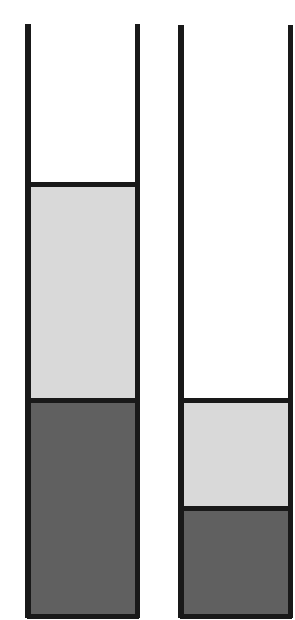
\includegraphics[scale=0.4]{figuurb.pdf}
                \caption{Illustration of a pure Nash equilibrium}
                \label{fig:b}
        \end{subfigure}
        \caption{(a) Illustration of the optimal assignment of an instance of the load balancing game with two large tasks of size 2 and two small tasks of size 1. The social cost of this assignment is 3. (b) Illustration of a pure Nash equilibrium for the same instance. The social cost of this assignment is 4, which is the maximum among all pure Nash equilibria for this instance.}
\end{figure}


\section{The Price of Anarchy}
\subsection{Definition}
Since players (`tasks') act selfishly, load balancing games may reach assignments that do not minimize the makespan. We now introduce the notion of the \emph{\textbf{price of the anarchy}} to quantify the degradation of the overall system performance.
\begin{definition}\cite{10}
Let \Nash(G) be the set of all (mixed) strategy profiles being a Nash equilibrium of a (load balancing) game $G$ and let $a_{\opt}$ be the pure strategy profile being the social optimum. Then the \emph{\textbf{price of anarchy}} is defined as:
$$PoA(G) = \displaystyle\max_{\alpha \in \Nash(G)} {\frac{\cost(\alpha)}{\cost(a_{\opt})}}$$
\end{definition}

The motivation behind studying the price of anarchy is to quantify the increase of the social cost due to selfish behavior. With this motivation in mind, does it makes more sense to consider pure or mixed Nash equilibria? Firstly, every load balancing game has a pure and mixed Nash equilibrium because it's a congestion and thus a strategy game. In reality, the answer depends: if one wants to study a distributed system in which tasks repeatedly perform improvement steps until they reach a Nash equilibrium, the situation of proof \ref{rosenthal} arises. However, there might be other means by which tasks come to a Nash equilibrium. Moreover, the upper bounds about the price of anarchy for mixed equilibria are more robust than upper bounds for pure equilibira as mixed equilibria are more general. We'll study both equilibria in two situations: the case in which all machines have an equal speed and the case they don't. It will be clear that if the machine speeds are relatively bounded an the number of task is large compared to the number of machines, then \emph{every Nash assignment approaches the social optimum}!

\subsection{Bachmann-Landau notations}
For understanding the four cases for which we'll study the price of the anarchy, it's important to know the \emph{Bachmann-Landau notations}. These notation are used to describe the limiting behavior of a function in terms of simpler functions. These notations are used a lot in computer science to classify algorithms by how they respond to change in input size.

\subsubsection{Bigh Oh, Big Omega \& Big Theta}
\begin{definition}\textbf{(Big Oh)}\cite{11}\\
Big Oh is the set of all functions $f$ that are bounded above by $g$ asymptotically (up to constant factor).
$$O(g(n)) = \{f|\exists c, n_0 \geq 0: \forall n \geq n_0 : 0 \leq f(n) \leq cg(n)\}$$
\end{definition}
We now proof a very simple lemma to show that indeed constant factors doesn't matter for Big Oh:
\begin{lemma}\label{constanten}
$\forall k > 0: O(k.g(n)) = O(g(n))$
\end{lemma}

\begin{proof}
\begin{eqnarray*}
O(k.g(n)) &=& \{f|\exists c, n_0 \geq 0: \forall n \geq n_0 : 0 \leq f(n) \leq k.c.g(n)\}\\
&=& \{f|\exists c, n_0 \geq 0: \forall n \geq n_0 : 0 \leq f(n) \leq (k.c).g(n)\}\\
\text{\small{let c' = k.c}}\\
&=& \{f|\exists c', n_0 \geq 0: \forall n \geq n_0 : 0 \leq f(n) \leq c'.g(n)\}\\
&=& O(g(n))
\end{eqnarray*}
\end{proof}


\begin{definition}\textbf{(Big Omega)}\cite{11}\\
Big Omega is the set of all functions $f$ that are bounded below by $g$ asymptotically (up to constant factor).
$$\Omega(g(n)) = \{f|\exists c, n_0 \geq 0: \forall n \geq n_0 : 0 \leq  cg(n)  \leq f(n) \}$$
\end{definition}
\begin{definition}\textbf{(Big Theta)}\cite{11}\\
Big Theta is the set of all functions $f$ that are bounded above and below by $g$ asymptotically (up to constant factors).
$$\Theta(g(n)) = \{f|\exists c_1, c_2 > 0, n_0 \geq 0: \forall n \geq n_0 : 0 \leq  c_1.g(n)  \leq f(n) \leq c_2.g(n)\}$$
\end{definition}

\subsubsection{Small Oh, Small Omega \& Small Theta}
\begin{definition}\textbf{(Small Oh)}\cite{12}\\
Small Oh is the set of all functions $f$ that are dominated by $g$ asymptotically.
$$o(g(n)) = \{f|\forall \varepsilon > 0, \exists n_0 \forall n \geq n_0: f(n) \leq \varepsilon.g(n)\}$$
\end{definition}
Equivalent definitions for small omega \& small theta can easily be found.  Note that the small oh-notation is a much stronger statement than the corresponding big oh-notation: every function that is in the small oh of $g$ is also in big oh, but the inverse isn't necessarily true. Intuitively, $f(x) \in o(g(x))$ means that $g(x)$ grows much faster than $f(x)$.

\subsubsection{Asymptotical Equality}
\begin{definition}\textbf{(Asymptotically Equal)}\cite{12}\\
Let $f$ and $g$ real functions, then $f$ is asymptotically equal to $g$ $\Leftrightarrow \displaystyle\lim_{x\rightarrow +\infty} \frac{f(x)}{g(x)}=1$. Notation: $f \sim g$.
\end{definition}
In fact asymptotical equality, can also be defined as an equivalency relation: $f\sim g \Leftrightarrow (f-g) \in o(g)$. It's trivially clear that as $f\sim g \Rightarrow f \in O(g)$.



\subsection{$PoA$ in Pure Nash Equilibria}
\subsubsection{Identical Machines}
\begin{theorem}\label{puurid}Let $G$ be a load balancing game with $n$ tasks of weight $w_1,...,w_n$ and $m$ identical machines. Under a pure Nash equilibrium $a \in A$ it holds:
$$\frac{cost(a)}{\cost(a_{\opt})} \leq 2 - \frac{2}{m+1}$$
\end{theorem}
\begin{proof}
Let $j^*$ be a machine with the highest load under profile $a$, and let $i*$ be a task of smallest weight assigned to this machine. WLOG, there are at least two tasks assigned to machine $j^*$ as, otherwise, $\cost(a) = \cost(a_{\opt})$ so that the upper bound given in the theorem follows trivially. Thus $w_{i^*} \leq \frac{1}{2}\cost(a)$.\\

Suppose there is a machine $j \in [m]\backslash{j^*}$ with load less than $l_{j^*}-w_{i^*}$. Then moving  the task $i^*$ from $j^*$ to $j$ would decrease the cost for this task. Hence, as $a$ is a Nash equilibrium it holds:
$$\ell_j \geq \ell_{j^*}-w_{i^*} \geq \cost(a) - \frac{1}{2}\cost(a) = \frac{1}{2}\cost(a).$$

Now observe that the cost of an optimal assignment cannot be smaller than the average load over all machines, so:
\begin{eqnarray*}
\copt           &\geq& \frac{\sum_{i \in [n]}w_i}{m}  \\
                &=&  \frac{\sum_{j \in [m]}\ell_j}{m}\\
                &\geq& \frac{cost(a) + \frac{1}{2}cost(a)(m-1)}{m}\\
                &=& \frac{(m+1)\cost(a)}{2m}
\end{eqnarray*}
\end{proof}
\subsubsection{Uniformly Related Machines}
We now switch from identical to uniformly related machines, i.e. machine $j$ has latency function $\ell_j(\alpha)$ (for a random mixed strategy profile $\alpha$). The analysis of the previous paragraph show that, in case of identical machines, the makespan of a pure Nash equilibrium is less than twice the optimal makespan. In this part, we show that the makespan of pure equilibria on uniformly related machines can deviate by more than a constant factor. The price of anarchy is bounded, however, by a slowly growing function in the number of machines.


\begin{figure}[t]
  \centering
  % Requires \usepackage{graphicx}
  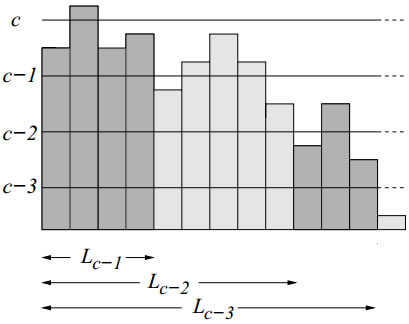
\includegraphics[scale=0.5]{lk.jpg}\\
  \caption{Illustration of the definition of the sets $L_{c-1}, L_{c-2},...L_0$ used in Definition \ref{lkdef}.}\label{lk}
\end{figure}

\begin{definition}\cite{4}\label{lkdef}
Let $L = [1,...,m]$ denote the list of machines in non-increasing order of speed (note that machines can always be re-ordered), and define $L_k$ as the maximum subset of $L$ such that the load of each machine in $L_k$ is at least $k.\copt$. Figure \ref{lk} illustrates the definition.
\end{definition}

\begin{lemma}\label{lemmalk}
Let $a^*$ be an optimal assignment, i.e. an assignment whose makespan is equal to $\copt$ and let $a$ denote a pure Nash equilibrium. Suppose $i$ is a task with $a(i) \in L_{k+1}$, then $a^*(i) \in L_k$.
\end{lemma}

\begin{proof}
If $L\setminus L_k = \emptyset$ then this claim follows trivially. Let $q$ be the smallest index in $L\setminus L_k$, i.e. machine $q$ is one of the machines with maximum speed among the machines $L\setminus L_k$. By definition of the group $L_k$, the load of $q$ is less than $k.\copt$, i.e., $\ell_q < k.\copt$. Figure \ref{lk2} illustrates the situation. \\
\begin{figure}
  \centering
  % Requires \usepackage{graphicx}
  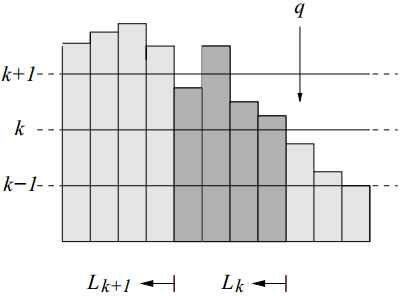
\includegraphics[scale=0.5]{lk2.jpg}\\
  \caption{Illustration of the sets $L_{k}$ and $L_{k+1}$ and the machine $q$ used in the proof of Lemma \ref{lemmalk}.}
  \label{lk2}
\end{figure}
By definition of the sets, $a(i) \in L_{k+1}$ implies $\ell_{a(i)} \geq (k+1).\copt$. Assume $w_i \leq s_q.\copt$. Moving task $i$ to machine $q$ would reduce the cost of $i$ to:
$$\ell_q + \frac{w_i}{s_q} < k.\copt + \copt \leq \ell_{a(i)},$$
which contradicts the assumption that $a$ is a pure Nash equilibrium. Hence, every task $i$ with $a(i) \in L_{k+1}$  satisfies $w_i > s_q.\copt$. Now, suppose $a^*(i) = j$ with $j \in L\setminus L_k$. Then the load on $j$ under $a^*$ would be at least
$$\frac{w_i}{s_j} > \frac{s_q.\copt}{s_j}\geq\copt$$
because $s_j \leq s_q$. However, this contradicts that $a^*$ is an optimal assignment. Consequently, $a^*(i) \in L_k$.
\end{proof}
$\Gamma^{-1}$ denotes the inverse of the \emph{gamma function}, an extension of the factorial function with the property that $\Gamma(k) = (k-1)!$, for every positive integer $k$. In the rest of this paper, the following property of $\Gamma^{-1}$ will be used several times:
\begin{lemma}\label{gamma}
$\forall m \in \R: \Gamma^{-1}(m) \in O\left(\frac{\log m}{\log \log m}\right)$.
\end{lemma}
\begin{proof}
Let $\Gamma^{-1}(m) = k$, then $k!$ is the greatest factorial smaller or equal to $m$, by definition of the (general) gamma function ($\Gamma(z) = \int_0^\infty  t^{z-1} e^{-t}\,{\rm d}t$). Because $m \sim k!$ and $k! \sim k^k$ we get:

\begin{eqnarray*}
&\Rightarrow& m \sim k^{k} \\
&\Rightarrow& \log m \sim k\log(k) \\
&\Rightarrow& k \sim \frac{\log m}{\log(k)}\\
&\Rightarrow& k \sim \frac{\log m}{\log(\frac{\log m}{\log (k)})}\\
&\Rightarrow& k \sim \frac{\log m}{\log\log m - \log\log (k)}
\end{eqnarray*}
Remember that, when using $O(...)$, constant factors don't matter by Definition \ref{constanten}, and any term that grows more slowly than another term can be abandoned by definition, because $m > k$:
$$\Rightarrow k \sim \frac{\log m}{\log \log m}$$

So that
$$\Gamma^{-1}(m) \in O\left(\frac{\log m}{\log \log m}\right)$$
\end{proof}

\begin{theorem}\label{puur}
Let $G$ be a load balancing game with $n$ tasks of weight $w_1,...,w_n$ and $m$ machines of speed $s_1, ..., s_m$. Let \emph{a} denote a pure Nash equilibrium. Then, it holds that:
$$\frac{cost(a)}{\cost(a_{\opt})} \in O\left(\frac{\log m}{\log \log m}\right)$$
\end{theorem}

\begin{proof}
Let $$c = \left\lfloor\frac{cost(\alpha)}{\cost(a_{\opt})}\right\rfloor.$$
We show $c \leq \Gamma^{-1}(m)$. This yields the theorem as in Lemma \ref{gamma}:
$$ \Gamma^{-1}(m) \in \Theta\left(\frac{\log m}{\log \log m}\right).$$
WLOG, let us assume $s_1 \geq s_2 \geq ... \geq s_m$ and let $L = [1,2,...,m]$ denote the list of machines in non-increasing order of speed. With definition \ref{lkdef} in mind, we will show the follow recurrence on the lengths of the sets $L_k$:
\begin{eqnarray*}
% \nonumber to remove numbering (before each equation)
  |L_k| &\geq& (k+1)|L_{k+1}|  \;\;\; \; (0\leq k \leq c-2)\\
  |L_{c-1}| &\geq& 1
\end{eqnarray*}
Solving the recurrence yields $|L_0| \geq (c-1)! = \Gamma(c)$. Now observe that $L_o = L$, and, hence, $|L_o| = m$. Consequently, $m \geq \Gamma(c)$ so that $c \leq \Gamma^{-1}(m)$, which proves the statement.\\

It remains to prove the recurrence. We first prove $|L_{c-1}| \geq 1$. Assume $L_{c-1} = \emptyset$, then the load of machine $1$ is less than $(c-1).\copt$. Moving $i$ to machine $1$ reduces the cost of $i$ to strictly less than
$$(c-1).\copt+\frac{w_i}{s_1} \leq (c-1).\copt + \copt \leq c.\copt$$
where the inequality $\frac{w_i}{s_1} \leq \copt$ follows from the fact that $s_1$ is the speed of the fastest machine. Consequently, player $i$ is able to unilaterally decrease its cost by moving its task from machine $j$ to machine $1$, which contradicts the assumption that $\alpha$ is a mixed Nash equilibrium. Thus, we have shown that $|L_{c-1}| \geq 1$.\\

Next, we show $|L_k| \geq (k+1)|L_{k+1}|$, for $0\leq k\leq c-2$. Let $a^*$ be an optimal assignment, i.e., an assignment whose makespan is equal to $\copt$. By definition of $L_{k+1}$, the sum of the weights that $a$ assigns to a machine $j \in L_{k+1}$ is at least $(k+1).\copt.s_j$. Hence, the total weight assigned to the machines in $L_{k+1}$ is at least $\sum_{j\in L_{k+1}}(k+1).\copt.s_j$. By lemma \ref{lemmalk} an optimal assignment has to assign all this weight to the machines in $L_k$ such that the load on each of these machines is at most $\copt$. As a consequence,

$$\displaystyle\sum_{j\in L_{k+1}}(k+1).\copt.s_j \leq \displaystyle\sum_{j\in L_k}\copt.s_j$$

Dividing by $\copt$ and substracting $\sum_{j\in L_{k+1}}s_j$ from both sides yields

$$\displaystyle\sum_{j\in L_{k+1}}k.s_j \leq \displaystyle\sum_{j\in L_k\setminus L_{k+1}}s_j$$

Now let $s^*$ denote the speed of the slowest machine in $L_{k+1}$, i.e., $s^*=s_{|L_{k+1}|}$. For all $j \in L_{k+1}$, $s_j\geq s^*$, and, for all $j \in L_k\setminus L_{k+1}, s_j\leq s^*$. Hence, we obtain
$$\displaystyle\sum_{j\in L_{k+1}}k.s^* \leq \sum_{j\in L_k\setminus L_{k+1}}s^*,$$
which implies $|L_{k+1}|.k \leq |L_k\setminus L_{k+1}| = |L_k|-|L_{k+1}|$. Thus, $|L_k| \geq (k+1).|L_{k+1}|$.
\end{proof}

We now prove a lower bound for the price of anarchy for pure Nash equilibria for uniformly related machines. This lower bound is important, because it shows us that the upper bound on the price of anarchy given in Theorem \ref{puur} is essentially tight.

\begin{theorem}\label{puur2}
For every $m \in \N$, there exists an instance of $G$ of the load balancing game with m machines and $n \leq m$ tasks that has a pure Nash equilibrium $a$ with:
$$\frac{cost(a)}{\cost(a_{\opt})} \in \Omega\left(\frac{\log m}{\log \log m}\right)$$
\end{theorem}
\begin{proof}
We will describe in this proof a game instance $G$ together with an equilibrium assignment $a$ satisfying
%NAKIJKEN!
$$\frac{cost(a)}{\cost(a_{\opt})} \geq \frac{1}{2} \left(\Gamma^{-1}(m) - 2 - o(1)\right)$$
which yields the theorem.
Our construction uses $q+1$ disjoint sets of machines denoted $G_0,...,G_q$ with $q \approx \Gamma^{-1}(m)$. More, precisely, we set
$$ q = \left\lfloor \Gamma^{-1}(\frac{m}{3}) - 1 \right\rfloor \geq \Gamma^{-1}(m)-2-o(1).$$
For $0 \leq k \leq q$, group $G_k$ consists of $q!/k!$ machines of speed $2^k$ each of which is assigned $k$ tasks of weight $2^k$. The total number of machines in these groups is thus:
$$\displaystyle\sum_{k=0}^{q} |G_k| = q! \displaystyle\sum_{k=0}^{q}\frac{1}{k!}\leq 3\Gamma(q+1) \leq m$$
because $\sum_{k=0}^{q}\frac{1}{k!} \leq 3$ and $3\Gamma(q+1)\leq m$, which follows directly from the definition of $q$. As $m$ might be larger than the number of the machines in the sets, there might be some machines that do not belong to any of the groups. We assume that these machines have the same parameters as the machines in group $G_0$: i.e., they have speed $2^0=1$ and $a$ does not assign tasks to them.\\
We need to show that the described assignment is a pure Nash equilibrium. A task on a machine from set $G_k$ has cost $k$. It can neither reduce its cost by moving its task to a machine in $G_j$ with $j\geq k$ as these machines have at least a load of $k$, nor can it reduce its cost by moving its task to a machine in group $G_j$ with $j < k$ as the load on such a machine, after the task moved to this machine, would be:
$$j + \frac{2^k}{2^j} = j + 2^{k-j} \geq j + (k - j + 1) = k + 1$$
since $2^t \geq t + 1$, for every $t\geq 1$. Hence, none of the tasks can unilaterally decrease its cost. In other words, $a$ is a pure Nash equilibrium.
The social cost or makespan of the equilibrium $a$ is $q$. Next, we show that $\copt \leq 2$ so that the theorem follows. We construct an assignment or strategy profile with load at moast $2$ on every machine. For each $k \in {1,...,q}$, the task mapped by $A$ to the machines in $G_k$ are now assigned tot the machines in $G_{k-1}$. Observe that the total number of tasks that $a$ maps to the machines in $G_k$ is
$$k|G_k| = k\frac{q!}{k!} = \frac{q!}{(k-1)!}= |G_{k-1}|.$$
Hence, we can assign the tasks in such a way that each machine in group $G_{k-1}$ receives exactly one of the tasks that $A$ mapped to a machine in group $G_k$. This task has a weight of $2^k$ and the speed of the machine is $2^{k-1}$. Hence, the load of each machine in this assignment is at most 2, which completes the proof.
\end{proof}
Theorem \ref{puur} gives an upper bound and Theorem \ref{puur2} gives a lower bound  for the price of anarchy for pure equilibria on uniformly related machines, so we conclude $\forall G$ with a pure equilibrium:
$$PoA(G) \in \Theta\left(\frac{\log m}{\log \log m}\right)$$



\subsection{$PoA$ in Mixed Nash Equilibria}
\subsubsection {Identical Machines}
In the following paragraph, we will prove a bound for the $PoA(G)$ for a mixed Nash Equilibrium. The proof uses the weighted Chernoff Bound theorem and Boole's inequality from probability theory. The weighted Chernoff Bound will not be proved in this paper.
\begin{theorem}\textbf{weighted Chernoff Bound}\label{chernoff}
Let $X_1,....X_n$ be independent random variables with values in the interval $[0,z]$ for some $z > 0$, and let $X = \sum^n_{i=1}X_i$, then for any $t$ it holds that $\P[\sum^n_{i=1}X_i\geq t] \leq (e.\E[X]/t)^{t/z}$.
\end{theorem}

\begin{theorem}\textbf{Boole's inequality}\cite{13}
For a countable set of events $A_1,...,A_n$ we have:
$$ \P\biggl(\bigcup_{i} A_i\biggr) \le \sum_i \P(A_i).$$
\end{theorem}
\begin{proof}
Boole's inequality may be proved using the method of induction.

For the $n=1$ case, it follows that
$\mathbb P(A_1) \le \mathbb P(A_1).$

For the case $n + 1$, we have
$$\P\biggl(\bigcup_{i=_1}^{n+1} A_i\biggr) \le \sum_{i=_1}^{n+1} \P(A_i).$$
Since $\mathbb P(A \cup B) = \mathbb P(A) + \mathbb P(B) - \mathbb P(A \cap B),$ and because the union operation is associative, we have
$$\P\biggl(\bigcup_{i=_1}^{n+1} A_i\biggr) = \P\biggl(\bigcup_{i=_1}^n A_i\biggr) + \mathbb P(A_{n+1}) - \P\biggl(\bigcup_{i=_1}^n A_i \cap A_{n+1}\biggr).$$
Since $\P\biggl(\bigcup_{i=_1}^n A_i \cap A_{n+1}\biggr) \ge 0$, as is the case for any probability measure, we have
$$\P\biggl(\bigcup_{i=_1}^{n+1} A_i\biggr) \le \P\biggl(\bigcup_{i=_1}^n A_i\biggr) + \mathbb P(A_{n+1})$$,
and therefore
$$\P\biggl(\bigcup_{i=_1}^{n+1} A_i\biggr) \le \sum_{i=_1}^{n} \P(A_i) + \mathbb P(A_{n+1}) = \sum_{i=_1}^{n+1} \P(A_i)$$.
\end{proof}


\begin{theorem}
Let $G$ be a load balancing game with $n$ tasks of weight $w_1,...,w_n$ and $m$ machines of equal speed. Let $\alpha$ denote a mixed Nash equilibrium. Then, it holds that:
$$\frac{cost(\alpha)}{\cost(a_{\opt})} \in O\left(\frac{\log m}{\log \log m}\right)$$
\end{theorem}

\begin{proof}
WLOG, we assume that all machines have speed $1$. Recall that $\cost(\alpha)=\E[\max_{j\in[m]}{\ell_j(a)}]$, i.e., $\cost(\alpha)$ corresponds to the expected maximum load over all machines. Our analysis starts with proving an upper bound on the maximum expected load instead of the expected maximum load.\\

We claim that, for every $j \in [m]: \ell_j(\alpha) \leq (2- \frac{2}{m+1})\copt$. The proof for this claim follows the course of the analyses for the upper bound on the price of anarchy for pure equilibria (with identical machines). More specifically, the proof of Theorem \ref{puurid} can be adapted as follows to mixed equilibria: instead of considering a smallest weight task $i^*$ placed on a maximum load machine $j^*$, one defines $i^*$ to be the smallest weight task with positive probability on a machine $j^*$ maximizing the expected load. Also in all other occurrences one considers the expected load instead of the load.\\

We conclude that the maximum expected load is less than $2.\copt$. Next we show that the expected maximum load deviates at most by a factor of $O(\frac{\log m}{\log \log m})$ from the maximum expected load. We use the weighted Chernoff bound in order to show that it is unlikely that there is a machine that deviates by a large factor from its expectation.

Fix $j \in [m]$. Let $w$ denote the largest weight of any task. Applying now the weighted Chernoff bound shows that, for every $t$,
$$\P[\ell_j \geq t] \leq \min\left\{1, \left(\frac{e.\E[\ell_j]}{t}\right)^{\frac{t}{w}} \right\}      \leq \left(\frac{2e\copt}{t}\right)^{t/\copt}.$$
because $\ell_j(\alpha) = \E[\ell_j]$, and $\ell_j(\alpha) \leq 2.\copt$ and $w \leq \copt$. Now let $\tau = 2\copt\frac{\ln m}{\ln \ln m}$. Then, for any $x \geq 0$,
\begin{eqnarray*}
\P[\ell_j \geq \tau + x] &\leq \left(\frac{e\ln\ln m}{\ln m}\right)^{2\frac{\ln m}{\ln \ln m} + \frac{x}{\copt}}\\
&\leq  \left(\frac{1}{\sqrt{\ln m}}\right)^{2\frac{\ln m}{\ln \ln m}}.e^{-\frac{x}{\copt}}\\
&= m^{-1}.e^{-\frac{x}{\copt}}
\end{eqnarray*}
where the second inequality holds asymptotically as, for sufficiently large $m$, $\frac{\ln m}{e \ln \ln m} \geq \sqrt{\log m}$ and $\frac{\ln m}{e \ln \ln m} \geq e$.\\
Now we can upper-bound $\cost(\alpha)$ as follows. For every nonnegative random variable $X$, $\E[X] = \int_0^\infty \P[X \geq t]dt$. Consequently,
$$\cost(\alpha) = \E\left[\max_{j\in[m]}\ell_j(a)\right] = \displaystyle\int_0^\infty{\P[\max_{j\in[m]}\ell_j(a) \geq t]}dt.$$
Substituting $t$ by $\tau + x$ and then applying the union bound yields:
$$\cost(\alpha) \leq \tau + \displaystyle\int_0^\infty{\P[\max_{j\in[m]}\ell_j(a) \geq \tau + x]}dx \leq
\displaystyle\int_0^\infty{\P[\ell_j(a) \geq \tau + x]}dx$$,
Finally, we apply the tail bound derived above and obtain
$$\cost(P) \leq \tau + \displaystyle\int_0^\infty{e^{\frac{-x}{\copt}}}dx = \tau + \copt,$$
which yields the theorem as $\tau = 2\copt\frac{\ln m}{\ln\ln m}.$

%tail bound!%
\end{proof}
From a purely mathematical point of view, it's necessary to proof also the lower bound in mixed Nash equilibria to conclude that $Pa(\alpha) \in \Theta(\frac{\log m}{\log \log m})$ for identical machines, but pure intuitively we can also use the fact that pure Nash equilibria reduce the level of anarchy, unlike mixed equilibria who increase the price. So, with Theorem \ref{puur2}, we conclude for mixed strategies on identical machines:
$$PoA(G) \in \Theta\left(\frac{\log m}{\log \log m}\right)$$

\subsubsection {Uniformly Related Machines}
Finally, we come to the most general case, namely mixed equilibria on uniformly related machines. The following theorem shows that the price of anarchy for this case is only slightly larger than the one for mixed equilibria on identical machines or pure equilibria on uniformly related machines.

For this purpose, we need two lemma's. Let $$c = \left\lfloor\max_{j\in[m]}\left(\frac{\E[\ell_j]}{s_j}\right)\right\rfloor$$ and remember Definition \ref{lkdef}. Choose $k \in [0, c-2]$ and define $G_k = L_k\setminus L_{k+1}$ and $G_{c-1}=L_{c-1}$. For $0 \leq k \leq c-1$, let $s(k)$ denote the speed of the fastest machine in $G_k$.

\begin{lemma}\label{geometrisch}
The sequence
$$s(c-1) \geq s(c-2) \geq ... \geq s(1) \geq s(0)$$
is geometrically decreasing or $s(k+2) \geq 2s(k) (for k \in {0,...,c-4})$.
\end{lemma}

\begin{proof}
Observe that there exists a task $j^*$ with $w_{j^*} \leq s(k+2)$ that has positive probability on a machine in $L_{k+3}$. This is because an optimal assignment strategy has to move some of the expected load from the machines in $L_{k+3}$ to machines in $L\setminus L_{k+3}$ and it can only assign those tasks to machines in $L\setminus L_{k+3}$ whose weights are not larger than the maximum speed among this set of machines, which is $s(k+2)$. Now suppose $s(k)>\frac{1}{2} s(k+2)$. The expected load of the fastest machine in $G_k = L_k\setminus L_{k+1}$ is at most $k+1$. Thus the expected cost of $j^*$ on the fastest machine in $G_k$ is at most
$$k+1 + \frac{w_{j^*}}{s(k)} < k + 1 + \frac{2w_{j^*}}{s(k+2)} \leq k+3.$$
This contradicts the expected cost of $j^*$ in the considered Nash equilibrium is at least $k+3$ as it has positive probability on machine $L_{k+3}$.
\end{proof}

For a machine $j \in [m]$, let $T_j^{(1)}$ denote the set of tasks $i$ with $\alpha_i(j) \geq \frac{1}{4}$ and $T_j^{(2)}$ the set of tasks $i$ with $\alpha_i(j) \in ]0, \frac{1}{4}[$.

\begin{lemma}\label{tj}
$$\forall j \in [m], \forall i \in T^{(2)}_j: w_i\leq 12s_j$$
\end{lemma}

\begin{proof}
Let $i$ be a task from $T^{(2)}_j$, i.e. $\alpha_i(j) \in ]0,\frac{1}{4}[$. Let $j \in G_k$, for $0\leq k \leq c-1$. The expected cost of $i$ on $j$ is:
$$U^j_i =\frac{\ell_j(\alpha) + (1 - \alpha_i(j))w_i }{s_j} \geq k + \frac{3w_i}{4s_j}.$$

Suppose that $k \geq c - 3$. In this case, $w_i > 12s_j$ implies $U_i^j > k + \frac{3}{4}.12 \geq c + 6$, which contradicts that, under the Nash equilibrium profile, the expected cost of any task on the fastest machine is at most $c + 1$. Hence, the lemma is shown for $k \geq c - 3$. Now suppose $k \leq c - 4$. Let $q$ denote the fastest machine from $G_{k+2}$. Lemma \ref{geometrisch} yields $s_q = s(k+2) \geq 2s(k) \geq 2s_j.$ Hence, the expected cost of $i$ on $q$ is
$$U_i^q = \frac{\ell_q(\alpha) + (1 - \alpha_i(q))w_i }{s_q}  \leq k + 3 + \frac{w_i}{2s_j}.$$
As $\alpha_i(j) > 0$, the Nash equilibrium condition yields $U_i^j \leq U_i^q$. Consequently,
$$k + \frac{3w_i}{4s_j} \leq k + 3 + \frac{w_i}{2s_j},$$
which implies $w_i \leq 12s_j.$
\end{proof}


\begin{theorem}\label{mei} Let $G$ be a load balancing game with $n$ tasks of weight $w_1,...,w_n$ and $m$ machines of speed $s_1,...,s_m$. Let $\alpha$ be any Nash equilibrium strategy profile. Then, it holds that:
$$\frac{cost(\alpha)}{\cost(a_{\opt})} \in O\left(\frac{\log m}{\log \log \log m}\right)$$
\end{theorem}
\begin{proof}
WLOG, assume $\copt$ = 1, which can be achieved by scaling the weights appropriately. We first prove bound on $c$ following the analysis for pure Nash equilibria in Theorem \ref{puur}. WLOG, assume $s_1 \geq s_2 \geq ... \geq s_m$. Let $L = [1,2,...,m]$ denote the list of machines in non increasing order of speed. Analogously to the analysis in the proof of Theorem \ref{puur}, one shows the recurrence $|L_k| \geq (k+1).|L_{k+1}|$, for $0 \leq k \leq c - 2$ and $|L_{c-1}| \geq 1$. Solving the recurrence yields $|L_0| \geq (c-1)! = \Gamma(c)$. Thus, $|L_0| = m$ implies $c \leq \Gamma^{-1}(m) = \Theta(\frac{\ln m}{\ln \ln m})$. Now let

$$C = \max\left\{c+1, \frac{\ln m}{\ln \ln m} \right\} = \Theta\left(\frac{\ln m}{\ln\ln m} \right)$$

In the rest of the proof, we show that the expected makespan of the equilibrium assignment can exceed $C$ at most by a factor of order $\ln\ln m/\ln \ln \ln m$ so that the expected makespan is $O(\ln m/\ln\ln\ln m)$, which proves the theorem as we assume $\copt = 1$.

As the next step, we prove a tail bound on $\frac{\ell_j(\alpha)}{s_j}$, for any fixed $j \in [m]$ and, afterward, we use this tail bound to derive an upper bound on the expected makespan.

Let $\ell_j^{(1)}$ and $\frac{\ell_j^{(2)}}{s_j}$ denote random variables that the describe the load on link $j$ only taking into account the tasks $T_j^{(1)}$ and $T_j^{(2)}$, respectively. Observe that $\frac{\ell_j(\alpha)}{s_j} = \frac{\ell_j^{(1)}(\alpha)}{s_j} + \frac{\ell_j^{(2)}(\alpha)}{s_j}$. For the tasks in $T_j^{(1)}$, we immediately obtain

\begin{equation}\label{equation1}
\frac{\ell_j^{(1)}}{s_j} \leq \displaystyle\sum_{i\in T_j^{(1)}}{\frac{w_i}{s_j}} \leq 4 \displaystyle\sum_{i\in T_j^{(1)}}{\frac{w_i p^j_i}{s_j}} = 4\E[\frac{\ell^(1)_j}{s_j}] \leq 4C.
\end{equation}

To prove an upper bound on $\frac{\ell_j^{(2)}}{s_j}$ , we use the weighted Chernoff bound from Lemma \ref{chernoff}. This bound requires an upper bound on the maximum weight. As a first step to bound the weights, we prove a result about the relationship between the speeds of the machines in the different groups that are defined by the prefixes. For $0 \leq k \leq c-2$, let $G_k = L_k\setminus L_{k+1}$, and let $G_{c-1}=L_{c-1}$. For $0 \leq k \leq c-1$, let $s(k)$ denote the speed of the fastest machine in $G_k$. By, Lemma \ref{geometrisch}, we know that this sequence is geometrically decreasing. Let $z=\max_{i\in T_j^{(2)}}(\frac{w_i}{s_j}$. Lemma \ref{tj} implies $z \leq 12$. Now applying the weighted Chernoff bound from Lemma \ref{chernoff} yields that, for every $\varphi > 0$

$$\P\left[\ell^{(2)}_j/s_j \geq \varphi C\right] \leq \left(\frac{e\E[\ell^{(2)}_j/s_j]}{\varphi C} \right) ^{\varphi C/z} \leq \left( \frac{e}{\varphi} \right)^{\varphi C/12} $$

since $\E[ \frac{\ell^{(2)}_j}{s_j}] \leq C.$ We define $\tau = 24C \ln\ln m/ \ln\ln\ln m$. As $C$ is of order $\ln m / \ln \ln m$, it follows that $\tau$ is of order $\ln m/ \ln\ln\ln m$. Let $x \geq 0$. We substitute $\tau + x$ for $\varphi C$ and obtain:
\begin{eqnarray*}
\P\left[\ell^{(2)}_j/s_j \geq \tau + x \right]  &\leq& \left(\frac{eC}{\tau+x} \right)\\
&\leq& \left(\frac{e \ln\ln\ln m}{24\ln\ln m} \right)^{2C\frac{\ln \ln m}{\ln\ln\ln m} + \frac{x}{12}}
\end{eqnarray*}

Observe that $24\ln\ln m/(e \ln\ln\ln m)$  is lower bounded by $\sqrt{\ln\ln m}$ and also lower bounded by $e^2$. Furthermore, $C \geq \ln m / \ln\ln m$. Applying these bounds yields

$$\P\left[\ell^{(2)}_j/s_j \geq \tau + x \right] \leq \left(\frac{1}{\sqrt{\ln \ln m}} \right)^{2\frac{\ln m}{\ln \ln \ln m}}.e^{-x/6} = m^{-1}.e^{-x/6}$$
As a consequence,
\begin{eqnarray*}
\E\left[\displaystyle\max_{j\in[m]}{\ell_j^{(2)}/s_j}\right] &=& \displaystyle\int^\infty_0{\P\left[\displaystyle\max_{j\in[m]}{\ell_j^{(2)}/s_j} \geq t  \right]dt}\\
&\leq& \tau + \displaystyle\int^\infty_0{\P\left[\displaystyle\max_{j\in[m]}{\ell_j^{(2)}/s_j} \geq \tau + x \right]dx} \\
&\leq& \tau + \displaystyle\int^\infty_0{\displaystyle\sum_{j\in[m]}\P\left[\ell_j^{(2)}/s_j  \geq \tau + x \right] dx}
\end{eqnarray*}
Now, applying our tail bound, yields
\begin{equation}\label{equation2}
\E\left[\displaystyle\max_{j\in[m]}{\ell_j^{(2)}/s_j}\right] \leq \tau + \displaystyle\int^\infty_0 e^{-x/6} dx = \tau + 6.
\end{equation}
Finally we combine equations \ref{equation1} and \ref{equation2} and obtain
$$\cost(\alpha) = \E\left[\displaystyle\max_{j\in[m]}{\ell_j^{(2)}/s_j}\right] \leq 4C + \tau + 6 = O\left(\frac{\log m}{\log \log \log m}\right)$$.
\end{proof}
Next, we show that the upper bound given in Theorem \ref{mei} is tight by showing that for every number of machines there exists a game instance that matches the upper bound up to a constant factor. We'll need an important result from combinatorics which we will not prove.

\begin{lemma}Suppose that $n \geq 1$ balls are placed independently, uniformly at random into $m \geq 1$ bins. then the expected maximum occupancy is
$$\Theta\left(\frac{\ln m}{\ln(1 + \frac{m}{n}\ln m} \right)$$
\end{lemma}\label{laatstelemma}


\begin{theorem}\label{mixed2}
For every $m \in \N$, there exists an instance $G$ of the load balancing game with $m$ machines and $n \leq m$ tasks that has a Nash equilibrium strategy profile $\alpha$ with:
$$\frac{\cost(\alpha)}{\copt} \in \Omega\left(\frac{\log m}{\log \log \log m} \right)$$
\end{theorem}

\begin{proof}
The starting point for our construction is the game and the pure Nash assignment $a$ from the proof of Theorem \ref{puur2}. We use mixed strategies in only one of the groups, namely in the group $G_k$ with $k = \lceil q/2 \rceil$. Let $M$ denote the number of machines in this group, i.e., $M = q!/k! \geq (q/2)^{\lfloor q/2 \rfloor}.$ Observe that $\log M \in \Theta(q \log q) = \Theta(\log m).$

Let $T$ denote the set of tasks mapped by $a$ to one of the machines in $G_k$. The tasks in $T$ have weight $2^k$. Each of these tasks is now assigned uniformly at random to a machine in group $G_k$, i.e., $\alpha_i(j)=\frac{1}{M}$, for each $j\in G_k$ and each $i \in T$. For all other tasks the new created mixed strategy $\alpha$ corresponds without any change to the pure strategy profile of assignment $a$. Observe that the randomization increases the expected costs of the tasks. The expected cost of a task $i\in T$ on a machine $j \in G_k$ is now
$$U_i^j = \frac{\ell_j(\alpha) + (1 - \alpha_i(j))w_i }{s_j} = k + \left(1 - \frac{1}{M}\right) < k+1.$$
In the proof of Theorem \ref{puur2}, we have shown that the cost of a task $i$ of weight $2^k$ on a machine of group $G_j$ with $j\neq k$ is at least $k+1$. Thus, the mixed strategy profile $\alpha$ is a Nash equilibrium.

It remains to compare the social cost of the equilibrium profile $\alpha$ with the optimal cost. The structure of the optimal assignment is not affected by the modifications. It has socials cost $\copt = 2$. Now we give a lower bound for the social cost of $\alpha$. This social cost is, obviously, bounded from below by the maximum number of tasks that are mapped to the same machine in the group $G_k$. Applying Lemma \ref{laatstelemma} with $M$ bins and $N = kM$ balls shows that the expected makespan is:
$$\Omega\left(\frac{\ln M}{\ln(1 + \frac{1}{k}\ln M)}\right) = \Omega\left(\frac{\log m}{\log\log\log m}\right),$$
where the last estimate holds as $k \in \Theta(\log m/\log \log m)$ and $\log M = \Theta(\log m)$. T
\end{proof}

Theorem \ref{mei} gives an upper bound and Theorem \ref{mixed2} gives a lower bound  for the price of anarchy for mixed equilibria on uniformly related machines, so we conclude $\forall G$ with an equilibrium:
$$PoA(G) \in \Theta\left(\frac{\log m}{\log \log \log m}\right)$$


\subsection{Summary}
The price of anarchy for pure and mixed Nash equilibria in load balancing games on identical and uniformly related machines can be summarized in this table:

\begin{center}
\begin{tabular}{l|c|c}

  % after \\: \hline or \cline{col1-col2} \cline{col3-col4} ...
   & Identical & Uniformly related \\
   \hline

   \hline
  Pure NE & $2-\frac{2}{m+1}$ & $\Theta\left(\frac{\log m}{\log \log m}\right)$ \\
  \hline
  Mixed NE & $\Theta\left(\frac{\log m}{\log \log m}\right)$ & $\Theta\left(\frac{\log m}{\log \log \log m}\right)$ \\
  \hline
\end{tabular}
\end{center}
\subsection{$PoA$ in Load Balancing Games with non-linear cost functions}
In section 4, we proved results that only apply on \emph{load balancing games} with \emph{linear cost functions} $c_j$ for each machine $j$ of the form: $c_j(x) = \lambda_jx+\mu_j$ (with $\lambda_j, \mu_j$ non-negative constants). Of course, cost function doesn't have to be linear at all, by example: $c_j(x) = \sqrt{\lambda_jx+\mu_j}$ or $c_j(x) =\lambda_jx^2+\mu_j$ are easy examples of functions who aren't. By studying this kind of load balancing games, it will be apparent that the price of anarchy is usally much worse than in the linear case. An extensive study of this kind of games falls behind the scope of this paper. However, note that in most cases the model with linear cost functions which is presented in this paper, can be applied by using linear regression.
\section{Coordination Mechanisms}
\subsection{Policies}
After building up the theory of the \emph{price of anarchy}, we now take a closer look to the $PoA$ in uniformly related machines. In the mixed and pure equilibrium case, we showed that $PoA \in  \Theta\left(\frac{\log m}{\log \log m}\right)$. Can we improve the $PoA$ by some `mechanism'? The mechanism should not only be easy to implement, but also, local to each machine. Consider the following rules for scheduling jobs on a machine:
\begin{itemize}
  \item \textbf{Shortest first}: a machine schedules the tasks on it in the order of increasing task weight.
  \item \textbf{Longest first}: a machine schedules the tasks on it in the order of decreasing task weight.
  \item \textbf{Random order}: a machine picks the tasks at random.
  \item \textbf{Round Robin}\cite{70}: Round-robin (RR) is a very simple scheduling algorithm for tasks. The principle is that time slices are assigned to each task in equal portions and in circular order, handling all tasks without priority. Round-robin is starvation-free.
\end{itemize}
Each rule above is a `policy'. Knowing the policy, the selfish tasks will behave differently. The important question is how the policy affects the $PoA$. Note that the game has changed in terms of the payoff functions. Each selfish task wants to finish as early as possible. Of course, this of course depends on the policy. The following theorems show (without proof) how a policy helps reducing $PoA$.

\begin{theorem} Under a longest-first policy, PoA for uniformly related machines is $\leq 2 - \frac{2}{m+1}$.
\end{theorem}

\begin{theorem} Under a shortest-first policy, PoA for uniformly related machines is $\Theta(\log m)$
\end{theorem}

We have to mention, that tasks (\emph{clients}) can cheat in the longest-first policy by stating that their task weight is longer than it actually is. It does not happen in the shortest first if we reasonably assume that a client would be unhappy if its task is left unprocessed. A mechanism is called \emph{truthful} if players have incentive to say their true value. Longest-first is in this sense not a truthful mechanism.

\subsection{Taxation}\cite{9}
In order to mititgate the effect of selfishness of the efficiency, recent research invented a solution with taxes: we assign taxes to machines. In this way, we obtain a new game where each task aims to minimize the sum of the latency he experiences and the tax he pays. Formally a \emph{tax function}: $\delta: M \times \R \rightarrow \R$ assigns a tax $\delta_j(w)$ to each task of weight $w$ that wishes to use machine $j \in M$. Furthermore, we assume that clients are not equally sensitive to taxes. In particular, task $i$ has a \emph{tax sensitivity} $\gamma_i > 0$. Assuming selfish behaviour of the clients, we obtain a new extended game $\langle G, \delta \rangle$ where each task now aims to minimize the expected cost he experiences plus his disutility due to the taxes he pays at the machine he uses. The disutility equals $\gamma_i \delta_j(w_i)$ when task $i$ selects machine $j$. Again, an assignment $a \in A$ is a pure Nash equilibrium for the extended game if no player has an incentive to unilaterally change his strategy, i.e. $\cost_i(a) + \gamma_i \delta_j(w_i) \leq \cost_i(a_{-i}, j^*) + \gamma_i \delta_{j^*}(w_i)$ for any task $i$ that is on machine $j$ under the assignment $a$. It can be shown that in this kind of extended games, the bounds on $PoA$ are better.
\newpage
\begin{thebibliography}{99}
\bibitem[BVOCK2007]{1} B. V\"{o}cking, \emph{Selfish Load Balancing}, Chapter 20 in Algorithmic Game Theory, Cambridge University Press, December 2007.
\bibitem[JOARU1994]{2} d J. Osborne and A. Rubinstein, \emph{A course in Game Theory},  The MIT Press, 1994.
\bibitem[MANN2008]{10} S. Mannor, \emph{Advancded Topics in Systems, Learning and Control, Lecture 3: Lecture 3: Mixed Actions, Nash and Correlated Equilibria}, Technicon, November 2008.
\bibitem[COL2011]{111} E. Colebunders, \emph{Analyse II}, Vrije Universiteit Brussel, 2011.
\bibitem[CW2007]{3} C. Witteveen, Intreerede: De Prijs van de Onafhankelijkheid, TU Delft 2007.
\bibitem[YMAN2003]{4} Y. Mansour, \emph{Lecture 6: Congestion and potential games}, Computational Learning Theory, University of Tel Aviv, 2003.
\bibitem[JMAR]{5} Jason R. Marden, \emph{Lecture 12: Game Theory Course}, University of Colorado.
\bibitem[THAR2011]{6} T. Harks, M. Klimm, R. H. M\"{o}hring, \emph{Characterizing the Existence of Potential Functions in Weighted Congestion Games}, February 2011
\bibitem[ROSENTHAL73]{7} R. W. Rosenthal, \emph{ A class of games possessing pure-strategy Nash equilibria}. International Journal of Game Theory, 2:65-67, 1973
\bibitem[ETE2007]{8} K. Etessami, \emph{Algorithmic Game Theory - Lecture 16 Best response dynamics and pure Nash Equilibria}, University of Edingburgh, 2007.

\bibitem[ICAR2008]{9} I. Caragiannis, C. Kaklamanis, P. Kanellopoulos, \emph{Improving the Efficiency of Load Balancing Games through Taxes}, University of Patras, 2008.

\bibitem[SUR2004]{10} S. Suri, C. D. T\'{o}th, Y. Zhou. \emph{Selfish Load Balancing and Atomic Congestion Games}, University of California, 2004.
\bibitem[MEU2011]{11} W. De Meuter. \emph{Algoritmen en Datastructuren I}, Vrije Universiteit Brussel, 2011.
\bibitem[BIN1977]{12} K.G. Binmore. \emph{Mathematical Analysis: A Straightforward Approach}, Cambridge Universitiy Press, 1977.
\bibitem[GAL1996]{13} Galambos, J\'{a}nos, Simonelli. \emph{Bonferroni-Type Inequalities with Applications, Probability and Its Applications}, Springer-Verlag, 1996.

\bibitem[SHI2008]{69} A. Shirazi, \emph{Algorithmic Game Theory: Coordination mechanisms},
University of Illinois, 2008.
\bibitem[SCH2011]{70} P. Schelkens, \emph{Syllabus: Computersystemen}, Vrije Universiteit Brussel, 2011.
    \end{thebibliography}
\end{document}

